\documentclass[xcolor={table}]{beamer}
\usepackage[size=a0,orientation=portrait,scale=1.55]{beamerposter}
\usepackage{graphicx}
\usepackage{caption}
\usepackage{subfigure}
\usepackage{siunitx}
%\usepackage{biblatex}
\usepackage{amsmath}
\usepackage{amsfonts}
\usepackage{amssymb}
\graphicspath{{images/}}


\begin{document}
\begin{frame}[fragile=singleslide,t]\centering

\begin{block}{WPT Architecture}
From the perspective of WPT, the end-to-end power transfer efficiency writes as:

\begin{equation}\label{eqn:power_utilization_efficiency}
  e = \frac{{{P_{{\text{dc}},{\text{ST}}}}}}{{P_{{\text{dc}}}^t}} = \underbrace {\frac{{P_{{\text{rf}}}^t}}{{P_{{\text{dc}}}^t}}}_{{e_1}} \cdot \underbrace {\frac{{P_{{\text{rf}}}^r}}{{P_{{\text{rf}}}^t}}}_{{e_2}} \cdot \underbrace {\frac{{P_{{\text{dc}}}^r}}{{P_{{\text{rf}}}^r}}}_{{e_3}} \cdot \underbrace {\frac{{{P_{{\text{dc}},{\text{ST}}}}}}{{P_{{\text{dc}}}^r}}}_{{e_4}}
\end{equation}

\begin{figure}
  \centering
    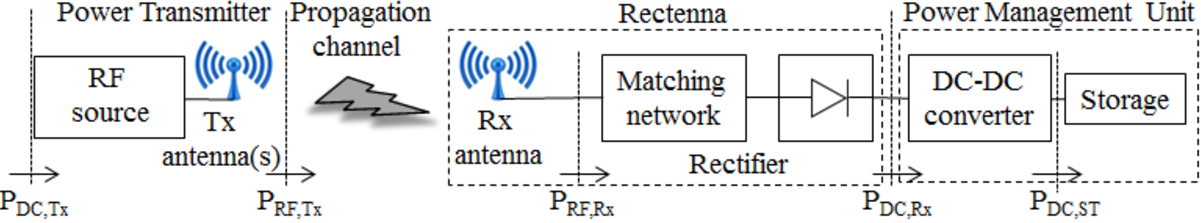
\includegraphics[width=0.9\textwidth]{wpt_block_diagram}
  \caption{Block diagram of a conventional far-field WPT architecture \cite{Clerckx2018a}. We particularly focus on the rectenna behavior.}
  \label{fig:wpt-block-diagram}
\end{figure}

The waveform design influences ${e_1}$, ${e_2}$ and ${e_3}$.
\end{block}

% The Diode Model
\begin{block}{The Diode Model}
\begin{equation}\label{eqn:current}
  {i_{\text{d}}}(t) = {i_{\text{s}}}\left( {{e^{\frac{{{v_{\text{d}}}(t)}}{{n{v_{\text{t}}}}}}} - 1} \right)\xrightarrow{{{\text{Taylor expansion}}}}{i_{\text{d}}}(t) = \sum\limits_{i = 0}^\infty  {k_i^\prime } {\left( {{v_{\text{d}}}(t) - a} \right)^i}\xrightarrow{{{\text{Expectation \&  Truncation}}}}{z_{DC}} = \sum\limits_{i{\text{ even,i}} \geqslant 2}^{{n_o}} {{k_i}} R_{{\text{ant}}}^{i/2}\mathbb{E}\left[ {y{{(t)}^i}} \right]
\end{equation}
\end{block}

% Rate-Energy Region
\begin{block}{Rate-Energy Region}
\begin{equation}\label{eqn:re_region}
  {C_{R - {I_{DC}}}}(P) \triangleq \left\{ {\left( {R,{I_{DC}}} \right):R \leqslant I,{I_{DC}} \leqslant {z_{DC}},\frac{1}{2}\left[ {\left\| {{{\mathbf{S}}_I}} \right\|_F^2 + \left\| {{{\mathbf{S}}_P}} \right\|_F^2} \right] \leqslant P} \right\}
\end{equation}
\end{block}

% Problem Formulation
\begin{block}{Problem Formulation}
We can convert the characterization of R-E region into an energy maximization problem with average transmit power budget $P$ and rate constraint ${\bar R}$
\begin{eqnarray}\label{eqn:problem}
  {\mathop {\max }\limits_{{{\mathbf{S}}_P},{{\mathbf{S}}_I},\rho } }&{{z_{DC}}\left( {{{\mathbf{S}}_P},{{\mathbf{S}}_I},{\mathbf{\Phi }}_P^ \star ,{\mathbf{\Phi }}_I^ \star ,\rho } \right)} \label{eqn:original_target}\\
  {{\text{ subject to }}}&{\frac{1}{2}\left[ {\left\| {{{\mathbf{S}}_I}} \right\|_F^2 + \left\| {{{\mathbf{S}}_P}} \right\|_F^2} \right] \leqslant P,} \label{eqn:original_power_constraint} \\
  {}&{I\left( {{{\mathbf{S}}_I},{\mathbf{\Phi }}_I^ \star ,\rho } \right) \geqslant \bar R} \label{eqn:original_rate_constraint}
\end{eqnarray}
The optimization can be transformed into standard Geometric Programming (GP) problems using Arithmetic Mean-Geometric Mean (AM-GM) inequality.
\end{block}

% Geometric Programming
\begin{block}{Geometric Programming}
\begin{itemize}
  \item Monomial: $g(x) = cx_1^{{a_1}}x_2^{{a_2}} \cdots x_n^{{a_n}},c > 0,{a_i} \in \mathbb{R}$
  \item Posynomial: $f(x) = \sum\limits_{k = 1}^K {{c_k}} x_1^{{a_{1k}}}x_2^{{a_{2k}}} \cdots x_n^{{a_{nk}}},{c_k} > 0$
  \item Signomial: $f(x) = \sum\limits_{k = 1}^K {{c_k}} x_1^{{a_{1k}}}x_2^{{a_{2k}}} \cdots x_n^{{a_{nk}}},{c_k} \in \mathbb{R}$
\end{itemize}
A standard GP is an optimization problem of the form
\begin{eqnarray}\label{eqn:gp}
  {{\text{minimize}}}&{{f_0}(x)} \\
  {{\text{subject to}}}&{{f_i}(x) \leqslant 1,\quad i = 1, \ldots ,m} \\
  {}&{{g_i}(x) = 1,\quad i = 1, \ldots ,p}
\end{eqnarray}
where ${{f_i}}$ are posynomial functions, ${{g_i}}$ are monomials, and ${{x_i}}$ are the optimization variables.
\end{block}

% AM-GM Inequality
\begin{block}{AM-GM Inequality}
The arithmetic mean of non-negative real numbers is greater than or equal to the geometric mean of the same list
\begin{equation}\label{eqn:am_gm}
  \frac{{{x_1} + {x_2} +  \cdots  + {x_n}}}{n} \geqslant \sqrt[n]{{{x_1}{x_2} \cdots {x_n}}}
\end{equation}
The transformation is based on a conservative approach to approximate the terms with posynomials in the denominator by new posynomials.
\end{block}

% Algorithms
\begin{block}{Algorithms}
\begin{itemize}
  \item Decoupling: guarantee the same performance by a joint space-frequency design with lower computational complexity
  \item Lower bound: the theoretical worst performance of the proposed design
  \item PAPR: practical constraint at the transmitter
  \item MIMO (suboptimal): consider the information and energy received in different rectennas
\end{itemize}
\end{block}

\bibliographystyle{IEEEtran}
\bibliography{library}

\end{frame}
\end{document} 